\section{Aufbau}
\label{sec:Aufbau}

In allen Versuchen werden ein Computer, eine Soundkarte, einen Lautsprecher und ein Mikrofon verwendet.
\subsection{Modellierung: Ein Teilchen im eindimensionalen Potential und im periodischen Festkörper}
Die Soundkarte wird an den Computer angeschlossen und mit einem auf einer Schiene befestigten Lautsprecher und einem auf dieser frei beweglichen Mikrofon verbunden. Zwischen Lautsprecher und Mikrofon werden Rohrstücke der Länge $\SI{25}{\milli\metre}$, $\SI{50}{\milli\metre}$ und $\SI{75}{\milli\metre}$ angeordnet, sodass eine auf beiden Seiten abgeschlossene Röhre entsteht.\\
Für den zweiten Versuchsteil werden zwischen den Rohrstücken Irisse mit $\SI{10}{\milli\metre}$, $\SI{13}{\milli\metre}$ und $\SI{16}{\milli\metre}$ Innendurchmesser angebracht.\newpage
\subsection{Modellierung: Das Wasserstoffatom}
Die an den Computer angeschlossene Soundkarte wird an Lautsprecher und Mikrofon in den zwei Hemisphären eines sphärischen Resonators angeschlossen, der in Abbildung \ref{fig:Res} zu sehen ist.
\begin{figure}
	\centering
	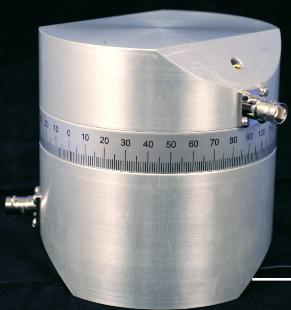
\includegraphics[scale=0.5]{content/images/Res.jpg}
	\caption{Sphärischer Resonator \cite{V23}.}
	\label{fig:Res}
\end{figure}

%╦ê♥
